\documentclass[12pt]{article}
\usepackage[table]{xcolor}
\usepackage[shortlabels]{enumitem}
\usepackage{tabularx,xltabular}
\usepackage{graphicx}
\usepackage{hyperref}
\usepackage{verbatim}
\usepackage{geometry}
\usepackage{ulem}
\usepackage[official]{eurosym}
\usepackage{tikz}
\usetikzlibrary{arrows,backgrounds,calc,decorations.markings,patterns,3d,positioning,fit,angles, quotes}
\usepackage{pgfplots}
\pgfplotsset{compat = newest}
\usetikzlibrary{fit}
\newcommand\addvmargin[1]{
\usetikzlibrary{arrows}
\node[fit=(current bounding box),inner ysep=#1,inner xsep=0]{};}
\usepackage{cancel}
\usepackage{fontspec}
\usepackage{array}  
\geometry{a4paper, top=2cm, left=2cm, right=2cm, bottom=2cm, headsep=1cm}
\usepackage{tabu}
\usepackage{pst-node}
\usepackage{colortbl}
\usepackage{array}
\usepackage{german}
\setlength\parindent{0pt}
\newcolumntype{?}{!{\vrule width 1pt}}
\usepackage{makecell}
\renewcommand{\arraystretch}{2.5}
\usepackage{pbox}
\usepackage{amssymb}
\usepackage{amsmath}
\usepackage{booktabs}
\newcolumntype{L}[1]{>{\raggedright\let\newline\\\arraybackslash\hspace{0pt}}m{#1}}
\newcolumntype{C}[1]{>{\centering\let\newline\\\arraybackslash\hspace{0pt}}m{#1}}
\newcolumntype{R}[1]{>{\raggedleft\let\newline\\\arraybackslash\hspace{0pt}}m{#1}}
\begin{document}
\rightline{Datum: 12.12.2023}
\centerline{{\Large Tägliche Übungen}} 
\vspace{1cm}
\noindent \\


\begin{xltabular}{\textwidth}{|C{0.75cm}|X|}
\arrayrulecolor{black}\hline
a)&\pbox{15cm}{
Welche Fläche ist größer, grün oder Blau?\\
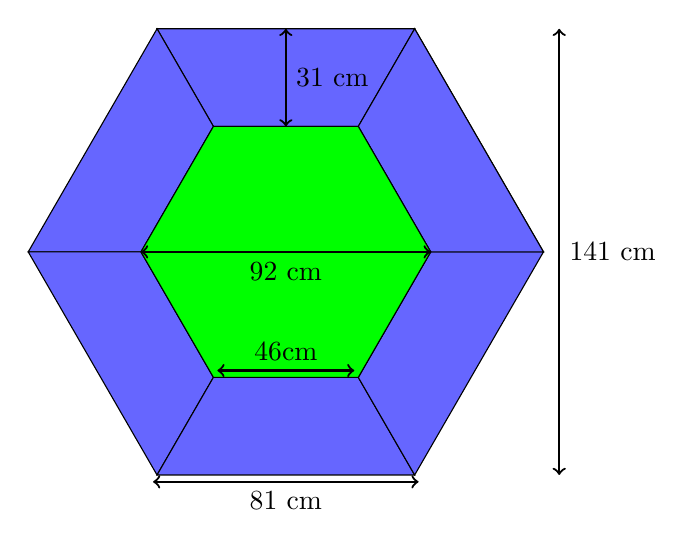
\begin{tikzpicture}
%Ich rechne mal sqrt(0.75) da hier ein gleichseitiges Dreieck vorliegt, bei dem man die Höhe berechnen muss.
%Dies geht mit dem Pythagoras, wobei der durch die Hälfte der Seite geht:
%               a²+b²=c² mit a=c/2 --> b²=c²-(c/2)²=c²-c²/4=3/4*c² --> b=c*sqrt(3/4)
%Flächenberechnung grün-blau in Python:
%R,h=50,25
%2*((2*R-R)*R*(0.75**0.5)/2)-6*((R+h*(0.75**0.5))-R)*h/2
  \pgfmathsetmacro{\hWert}{31}
  \pgfmathsetmacro{\RWert}{46}
  \pgfmathsetmacro{\dh}{\hWert/100*4}
  \pgfmathsetmacro{\R}{\RWert/100*4}
  \pgfmathsetmacro{\dR}{\dh/sqrt(0.75)}
  \pgfmathsetmacro{\hges}{(\R+\dR)*sqrt(0.75)}
  \pgfmathsetmacro{\h}{\hges-\dh}
%Schreibe ohne Komma
  \pgfmathtruncatemacro\gesamthoehe{2*(\RWert*sqrt(0.75)+\hWert)}
  \pgfmathtruncatemacro\aussenlaenge{\RWert+\hWert/sqrt(0.75)}
  \pgfmathtruncatemacro\innenlaenge{2*\RWert}
  \pgfmathtruncatemacro\innenhoehe{\RWert*sqrt(0.75)}
\foreach \rot in  {0,60,...,360}{
\draw[black,rotate=\rot,fill=blue!60] (\R,0) -- ++(\dR,0) -- ++(120:\R+\dR) -- ++(60:-\dR) -- cycle;
}
\draw[black,fill=green] (\R,0) -- ++(120:\R) -- ++(180:\R) -- ++(240:\R) -- ++(120:-\R) -- ++(0:\R) -- cycle ;
\draw[thick,<->] (-\R,0) --node[below] {\innenlaenge~cm} (\R,0);
\draw[thick,<->] (\R+\dR+0.2,\hges) --node[right] {\gesamthoehe~cm} (\R+\dR+0.2,-\hges) ;
\draw[thick,<->] (240:\R-0.1) --node[above] {\RWert cm}  (300:\R-0.1);
\draw[thick,<->] (240:\R+\dR+0.1) --node[below] {\aussenlaenge~cm}  (300:\R+\dR+0.1);
\draw[thick,<->] (0,\h) --node[right] {\hWert~cm} (0,\hges);
\end{tikzpicture}
}
\\\hline
b)&\pbox{15cm}{
Welche Fläche ist größer, grün oder Blau?\\
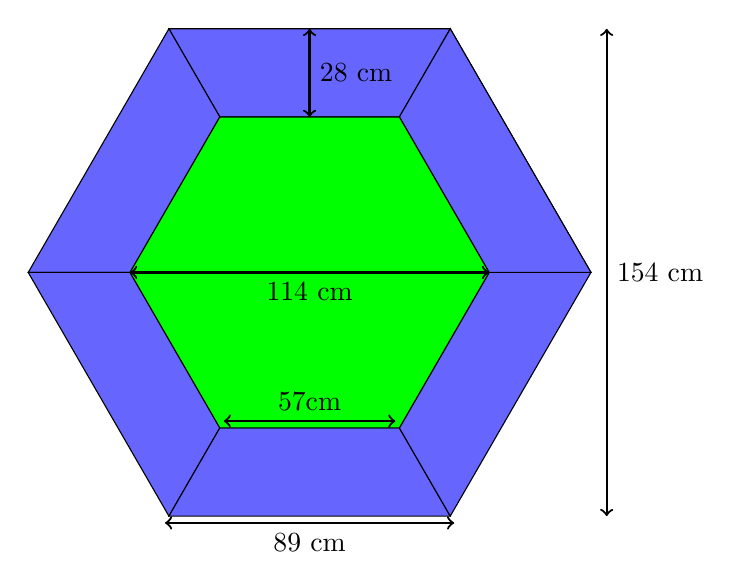
\begin{tikzpicture}
%Ich rechne mal sqrt(0.75) da hier ein gleichseitiges Dreieck vorliegt, bei dem man die Höhe berechnen muss.
%Dies geht mit dem Pythagoras, wobei der durch die Hälfte der Seite geht:
%               a²+b²=c² mit a=c/2 --> b²=c²-(c/2)²=c²-c²/4=3/4*c² --> b=c*sqrt(3/4)
%Flächenberechnung grün-blau in Python:
%R,h=50,25
%2*((2*R-R)*R*(0.75**0.5)/2)-6*((R+h*(0.75**0.5))-R)*h/2
  \pgfmathsetmacro{\hWert}{28}
  \pgfmathsetmacro{\RWert}{57}
  \pgfmathsetmacro{\dh}{\hWert/100*4}
  \pgfmathsetmacro{\R}{\RWert/100*4}
  \pgfmathsetmacro{\dR}{\dh/sqrt(0.75)}
  \pgfmathsetmacro{\hges}{(\R+\dR)*sqrt(0.75)}
  \pgfmathsetmacro{\h}{\hges-\dh}
%Schreibe ohne Komma
  \pgfmathtruncatemacro\gesamthoehe{2*(\RWert*sqrt(0.75)+\hWert)}
  \pgfmathtruncatemacro\aussenlaenge{\RWert+\hWert/sqrt(0.75)}
  \pgfmathtruncatemacro\innenlaenge{2*\RWert}
  \pgfmathtruncatemacro\innenhoehe{\RWert*sqrt(0.75)}
\foreach \rot in  {0,60,...,360}{
\draw[black,rotate=\rot,fill=blue!60] (\R,0) -- ++(\dR,0) -- ++(120:\R+\dR) -- ++(60:-\dR) -- cycle;
}
\draw[black,fill=green] (\R,0) -- ++(120:\R) -- ++(180:\R) -- ++(240:\R) -- ++(120:-\R) -- ++(0:\R) -- cycle ;
\draw[thick,<->] (-\R,0) --node[below] {\innenlaenge~cm} (\R,0);
\draw[thick,<->] (\R+\dR+0.2,\hges) --node[right] {\gesamthoehe~cm} (\R+\dR+0.2,-\hges) ;
\draw[thick,<->] (240:\R-0.1) --node[above] {\RWert cm}  (300:\R-0.1);
\draw[thick,<->] (240:\R+\dR+0.1) --node[below] {\aussenlaenge~cm}  (300:\R+\dR+0.1);
\draw[thick,<->] (0,\h) --node[right] {\hWert~cm} (0,\hges);
\end{tikzpicture}
}
\\\hline
c)&\pbox{15cm}{
Welche Fläche ist größer, grün oder Blau?\\
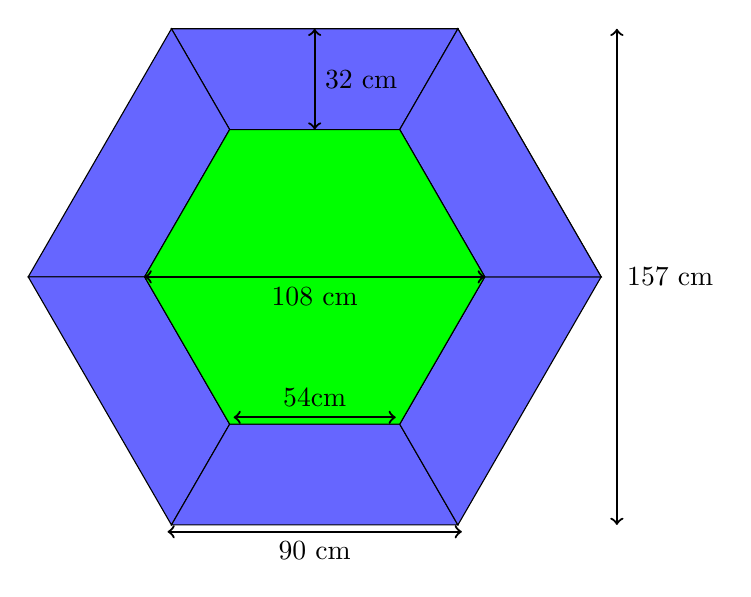
\begin{tikzpicture}
%Ich rechne mal sqrt(0.75) da hier ein gleichseitiges Dreieck vorliegt, bei dem man die Höhe berechnen muss.
%Dies geht mit dem Pythagoras, wobei der durch die Hälfte der Seite geht:
%               a²+b²=c² mit a=c/2 --> b²=c²-(c/2)²=c²-c²/4=3/4*c² --> b=c*sqrt(3/4)
%Flächenberechnung grün-blau in Python:
%R,h=50,25
%2*((2*R-R)*R*(0.75**0.5)/2)-6*((R+h*(0.75**0.5))-R)*h/2
  \pgfmathsetmacro{\hWert}{32}
  \pgfmathsetmacro{\RWert}{54}
  \pgfmathsetmacro{\dh}{\hWert/100*4}
  \pgfmathsetmacro{\R}{\RWert/100*4}
  \pgfmathsetmacro{\dR}{\dh/sqrt(0.75)}
  \pgfmathsetmacro{\hges}{(\R+\dR)*sqrt(0.75)}
  \pgfmathsetmacro{\h}{\hges-\dh}
%Schreibe ohne Komma
  \pgfmathtruncatemacro\gesamthoehe{2*(\RWert*sqrt(0.75)+\hWert)}
  \pgfmathtruncatemacro\aussenlaenge{\RWert+\hWert/sqrt(0.75)}
  \pgfmathtruncatemacro\innenlaenge{2*\RWert}
  \pgfmathtruncatemacro\innenhoehe{\RWert*sqrt(0.75)}
\foreach \rot in  {0,60,...,360}{
\draw[black,rotate=\rot,fill=blue!60] (\R,0) -- ++(\dR,0) -- ++(120:\R+\dR) -- ++(60:-\dR) -- cycle;
}
\draw[black,fill=green] (\R,0) -- ++(120:\R) -- ++(180:\R) -- ++(240:\R) -- ++(120:-\R) -- ++(0:\R) -- cycle ;
\draw[thick,<->] (-\R,0) --node[below] {\innenlaenge~cm} (\R,0);
\draw[thick,<->] (\R+\dR+0.2,\hges) --node[right] {\gesamthoehe~cm} (\R+\dR+0.2,-\hges) ;
\draw[thick,<->] (240:\R-0.1) --node[above] {\RWert cm}  (300:\R-0.1);
\draw[thick,<->] (240:\R+\dR+0.1) --node[below] {\aussenlaenge~cm}  (300:\R+\dR+0.1);
\draw[thick,<->] (0,\h) --node[right] {\hWert~cm} (0,\hges);
\end{tikzpicture}
}
\\\hline
d)&\pbox{15cm}{
Welche Fläche ist größer, grün oder Blau?\\
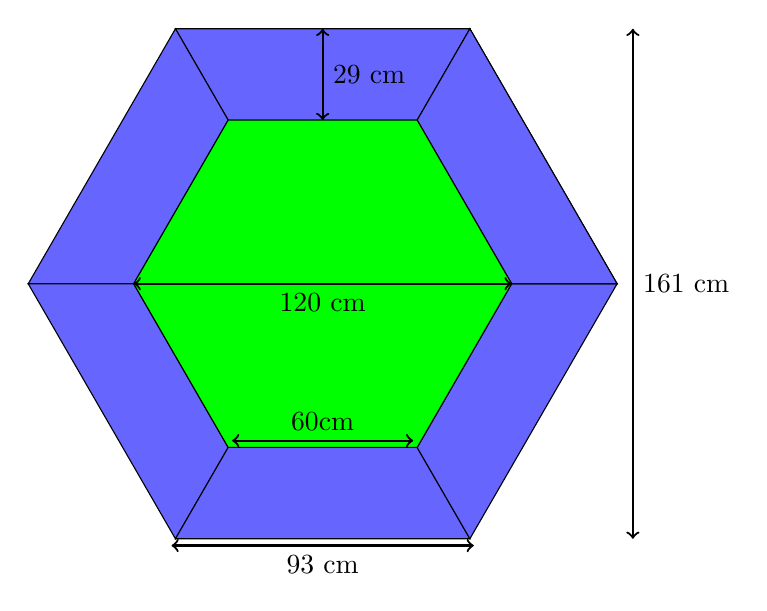
\begin{tikzpicture}
%Ich rechne mal sqrt(0.75) da hier ein gleichseitiges Dreieck vorliegt, bei dem man die Höhe berechnen muss.
%Dies geht mit dem Pythagoras, wobei der durch die Hälfte der Seite geht:
%               a²+b²=c² mit a=c/2 --> b²=c²-(c/2)²=c²-c²/4=3/4*c² --> b=c*sqrt(3/4)
%Flächenberechnung grün-blau in Python:
%R,h=50,25
%2*((2*R-R)*R*(0.75**0.5)/2)-6*((R+h*(0.75**0.5))-R)*h/2
  \pgfmathsetmacro{\hWert}{29}
  \pgfmathsetmacro{\RWert}{60}
  \pgfmathsetmacro{\dh}{\hWert/100*4}
  \pgfmathsetmacro{\R}{\RWert/100*4}
  \pgfmathsetmacro{\dR}{\dh/sqrt(0.75)}
  \pgfmathsetmacro{\hges}{(\R+\dR)*sqrt(0.75)}
  \pgfmathsetmacro{\h}{\hges-\dh}
%Schreibe ohne Komma
  \pgfmathtruncatemacro\gesamthoehe{2*(\RWert*sqrt(0.75)+\hWert)}
  \pgfmathtruncatemacro\aussenlaenge{\RWert+\hWert/sqrt(0.75)}
  \pgfmathtruncatemacro\innenlaenge{2*\RWert}
  \pgfmathtruncatemacro\innenhoehe{\RWert*sqrt(0.75)}
\foreach \rot in  {0,60,...,360}{
\draw[black,rotate=\rot,fill=blue!60] (\R,0) -- ++(\dR,0) -- ++(120:\R+\dR) -- ++(60:-\dR) -- cycle;
}
\draw[black,fill=green] (\R,0) -- ++(120:\R) -- ++(180:\R) -- ++(240:\R) -- ++(120:-\R) -- ++(0:\R) -- cycle ;
\draw[thick,<->] (-\R,0) --node[below] {\innenlaenge~cm} (\R,0);
\draw[thick,<->] (\R+\dR+0.2,\hges) --node[right] {\gesamthoehe~cm} (\R+\dR+0.2,-\hges) ;
\draw[thick,<->] (240:\R-0.1) --node[above] {\RWert cm}  (300:\R-0.1);
\draw[thick,<->] (240:\R+\dR+0.1) --node[below] {\aussenlaenge~cm}  (300:\R+\dR+0.1);
\draw[thick,<->] (0,\h) --node[right] {\hWert~cm} (0,\hges);
\end{tikzpicture}
}
\\\hline
e)&\pbox{15cm}{
Welche Fläche ist größer, grün oder Blau?\\
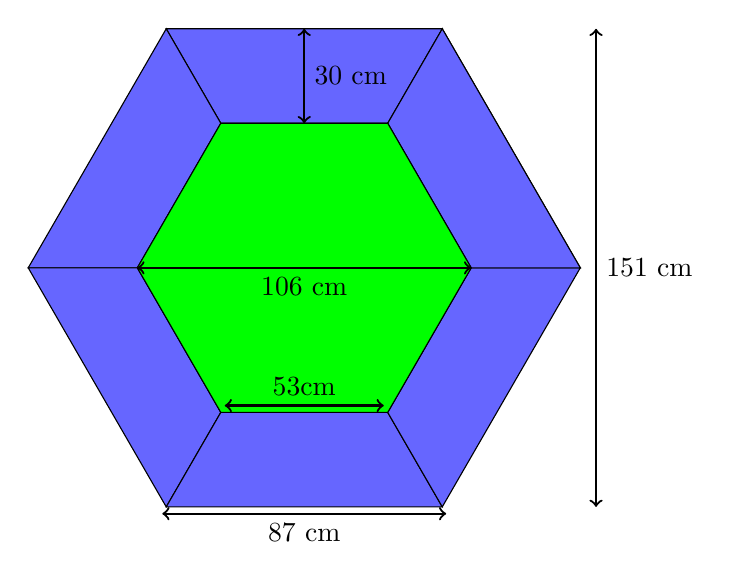
\begin{tikzpicture}
%Ich rechne mal sqrt(0.75) da hier ein gleichseitiges Dreieck vorliegt, bei dem man die Höhe berechnen muss.
%Dies geht mit dem Pythagoras, wobei der durch die Hälfte der Seite geht:
%               a²+b²=c² mit a=c/2 --> b²=c²-(c/2)²=c²-c²/4=3/4*c² --> b=c*sqrt(3/4)
%Flächenberechnung grün-blau in Python:
%R,h=50,25
%2*((2*R-R)*R*(0.75**0.5)/2)-6*((R+h*(0.75**0.5))-R)*h/2
  \pgfmathsetmacro{\hWert}{30}
  \pgfmathsetmacro{\RWert}{53}
  \pgfmathsetmacro{\dh}{\hWert/100*4}
  \pgfmathsetmacro{\R}{\RWert/100*4}
  \pgfmathsetmacro{\dR}{\dh/sqrt(0.75)}
  \pgfmathsetmacro{\hges}{(\R+\dR)*sqrt(0.75)}
  \pgfmathsetmacro{\h}{\hges-\dh}
%Schreibe ohne Komma
  \pgfmathtruncatemacro\gesamthoehe{2*(\RWert*sqrt(0.75)+\hWert)}
  \pgfmathtruncatemacro\aussenlaenge{\RWert+\hWert/sqrt(0.75)}
  \pgfmathtruncatemacro\innenlaenge{2*\RWert}
  \pgfmathtruncatemacro\innenhoehe{\RWert*sqrt(0.75)}
\foreach \rot in  {0,60,...,360}{
\draw[black,rotate=\rot,fill=blue!60] (\R,0) -- ++(\dR,0) -- ++(120:\R+\dR) -- ++(60:-\dR) -- cycle;
}
\draw[black,fill=green] (\R,0) -- ++(120:\R) -- ++(180:\R) -- ++(240:\R) -- ++(120:-\R) -- ++(0:\R) -- cycle ;
\draw[thick,<->] (-\R,0) --node[below] {\innenlaenge~cm} (\R,0);
\draw[thick,<->] (\R+\dR+0.2,\hges) --node[right] {\gesamthoehe~cm} (\R+\dR+0.2,-\hges) ;
\draw[thick,<->] (240:\R-0.1) --node[above] {\RWert cm}  (300:\R-0.1);
\draw[thick,<->] (240:\R+\dR+0.1) --node[below] {\aussenlaenge~cm}  (300:\R+\dR+0.1);
\draw[thick,<->] (0,\h) --node[right] {\hWert~cm} (0,\hges);
\end{tikzpicture}
}
\\\hline
f)&\pbox{15cm}{
Welche Fläche ist größer, grün oder Blau?\\
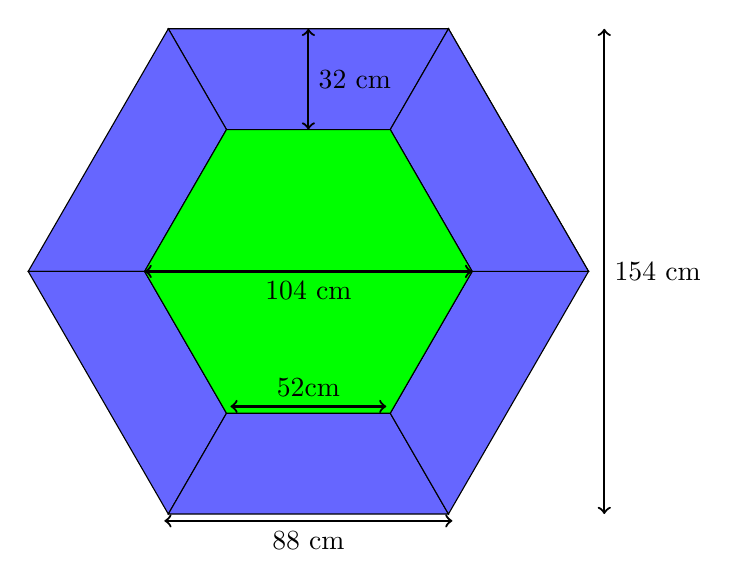
\begin{tikzpicture}
%Ich rechne mal sqrt(0.75) da hier ein gleichseitiges Dreieck vorliegt, bei dem man die Höhe berechnen muss.
%Dies geht mit dem Pythagoras, wobei der durch die Hälfte der Seite geht:
%               a²+b²=c² mit a=c/2 --> b²=c²-(c/2)²=c²-c²/4=3/4*c² --> b=c*sqrt(3/4)
%Flächenberechnung grün-blau in Python:
%R,h=50,25
%2*((2*R-R)*R*(0.75**0.5)/2)-6*((R+h*(0.75**0.5))-R)*h/2
  \pgfmathsetmacro{\hWert}{32}
  \pgfmathsetmacro{\RWert}{52}
  \pgfmathsetmacro{\dh}{\hWert/100*4}
  \pgfmathsetmacro{\R}{\RWert/100*4}
  \pgfmathsetmacro{\dR}{\dh/sqrt(0.75)}
  \pgfmathsetmacro{\hges}{(\R+\dR)*sqrt(0.75)}
  \pgfmathsetmacro{\h}{\hges-\dh}
%Schreibe ohne Komma
  \pgfmathtruncatemacro\gesamthoehe{2*(\RWert*sqrt(0.75)+\hWert)}
  \pgfmathtruncatemacro\aussenlaenge{\RWert+\hWert/sqrt(0.75)}
  \pgfmathtruncatemacro\innenlaenge{2*\RWert}
  \pgfmathtruncatemacro\innenhoehe{\RWert*sqrt(0.75)}
\foreach \rot in  {0,60,...,360}{
\draw[black,rotate=\rot,fill=blue!60] (\R,0) -- ++(\dR,0) -- ++(120:\R+\dR) -- ++(60:-\dR) -- cycle;
}
\draw[black,fill=green] (\R,0) -- ++(120:\R) -- ++(180:\R) -- ++(240:\R) -- ++(120:-\R) -- ++(0:\R) -- cycle ;
\draw[thick,<->] (-\R,0) --node[below] {\innenlaenge~cm} (\R,0);
\draw[thick,<->] (\R+\dR+0.2,\hges) --node[right] {\gesamthoehe~cm} (\R+\dR+0.2,-\hges) ;
\draw[thick,<->] (240:\R-0.1) --node[above] {\RWert cm}  (300:\R-0.1);
\draw[thick,<->] (240:\R+\dR+0.1) --node[below] {\aussenlaenge~cm}  (300:\R+\dR+0.1);
\draw[thick,<->] (0,\h) --node[right] {\hWert~cm} (0,\hges);
\end{tikzpicture}
}
\\\hline
g)&\pbox{15cm}{
Welche Fläche ist größer, grün oder Blau?\\
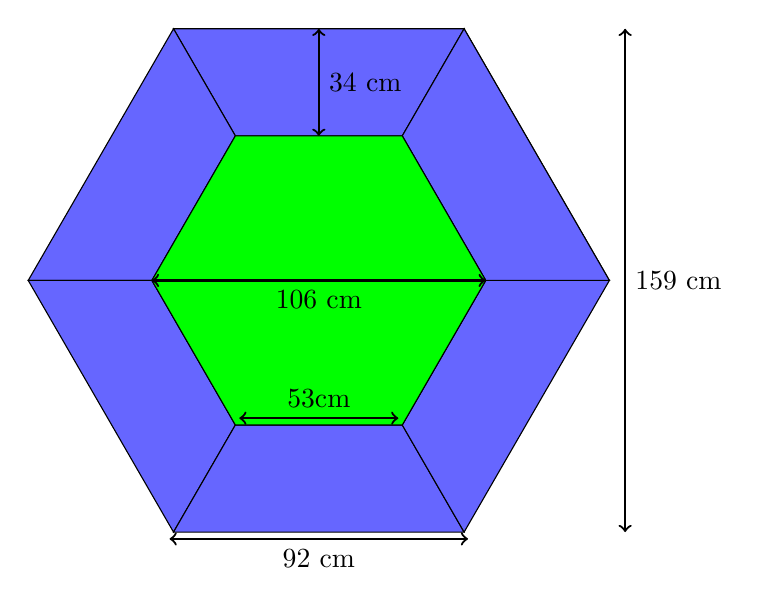
\begin{tikzpicture}
%Ich rechne mal sqrt(0.75) da hier ein gleichseitiges Dreieck vorliegt, bei dem man die Höhe berechnen muss.
%Dies geht mit dem Pythagoras, wobei der durch die Hälfte der Seite geht:
%               a²+b²=c² mit a=c/2 --> b²=c²-(c/2)²=c²-c²/4=3/4*c² --> b=c*sqrt(3/4)
%Flächenberechnung grün-blau in Python:
%R,h=50,25
%2*((2*R-R)*R*(0.75**0.5)/2)-6*((R+h*(0.75**0.5))-R)*h/2
  \pgfmathsetmacro{\hWert}{34}
  \pgfmathsetmacro{\RWert}{53}
  \pgfmathsetmacro{\dh}{\hWert/100*4}
  \pgfmathsetmacro{\R}{\RWert/100*4}
  \pgfmathsetmacro{\dR}{\dh/sqrt(0.75)}
  \pgfmathsetmacro{\hges}{(\R+\dR)*sqrt(0.75)}
  \pgfmathsetmacro{\h}{\hges-\dh}
%Schreibe ohne Komma
  \pgfmathtruncatemacro\gesamthoehe{2*(\RWert*sqrt(0.75)+\hWert)}
  \pgfmathtruncatemacro\aussenlaenge{\RWert+\hWert/sqrt(0.75)}
  \pgfmathtruncatemacro\innenlaenge{2*\RWert}
  \pgfmathtruncatemacro\innenhoehe{\RWert*sqrt(0.75)}
\foreach \rot in  {0,60,...,360}{
\draw[black,rotate=\rot,fill=blue!60] (\R,0) -- ++(\dR,0) -- ++(120:\R+\dR) -- ++(60:-\dR) -- cycle;
}
\draw[black,fill=green] (\R,0) -- ++(120:\R) -- ++(180:\R) -- ++(240:\R) -- ++(120:-\R) -- ++(0:\R) -- cycle ;
\draw[thick,<->] (-\R,0) --node[below] {\innenlaenge~cm} (\R,0);
\draw[thick,<->] (\R+\dR+0.2,\hges) --node[right] {\gesamthoehe~cm} (\R+\dR+0.2,-\hges) ;
\draw[thick,<->] (240:\R-0.1) --node[above] {\RWert cm}  (300:\R-0.1);
\draw[thick,<->] (240:\R+\dR+0.1) --node[below] {\aussenlaenge~cm}  (300:\R+\dR+0.1);
\draw[thick,<->] (0,\h) --node[right] {\hWert~cm} (0,\hges);
\end{tikzpicture}
}
\\\hline
h)&\pbox{15cm}{
Welche Fläche ist größer, grün oder Blau?\\
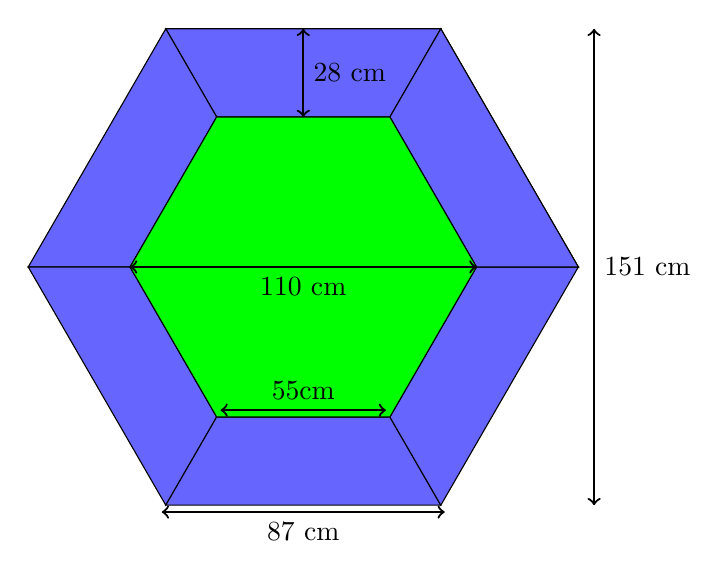
\begin{tikzpicture}
%Ich rechne mal sqrt(0.75) da hier ein gleichseitiges Dreieck vorliegt, bei dem man die Höhe berechnen muss.
%Dies geht mit dem Pythagoras, wobei der durch die Hälfte der Seite geht:
%               a²+b²=c² mit a=c/2 --> b²=c²-(c/2)²=c²-c²/4=3/4*c² --> b=c*sqrt(3/4)
%Flächenberechnung grün-blau in Python:
%R,h=50,25
%2*((2*R-R)*R*(0.75**0.5)/2)-6*((R+h*(0.75**0.5))-R)*h/2
  \pgfmathsetmacro{\hWert}{28}
  \pgfmathsetmacro{\RWert}{55}
  \pgfmathsetmacro{\dh}{\hWert/100*4}
  \pgfmathsetmacro{\R}{\RWert/100*4}
  \pgfmathsetmacro{\dR}{\dh/sqrt(0.75)}
  \pgfmathsetmacro{\hges}{(\R+\dR)*sqrt(0.75)}
  \pgfmathsetmacro{\h}{\hges-\dh}
%Schreibe ohne Komma
  \pgfmathtruncatemacro\gesamthoehe{2*(\RWert*sqrt(0.75)+\hWert)}
  \pgfmathtruncatemacro\aussenlaenge{\RWert+\hWert/sqrt(0.75)}
  \pgfmathtruncatemacro\innenlaenge{2*\RWert}
  \pgfmathtruncatemacro\innenhoehe{\RWert*sqrt(0.75)}
\foreach \rot in  {0,60,...,360}{
\draw[black,rotate=\rot,fill=blue!60] (\R,0) -- ++(\dR,0) -- ++(120:\R+\dR) -- ++(60:-\dR) -- cycle;
}
\draw[black,fill=green] (\R,0) -- ++(120:\R) -- ++(180:\R) -- ++(240:\R) -- ++(120:-\R) -- ++(0:\R) -- cycle ;
\draw[thick,<->] (-\R,0) --node[below] {\innenlaenge~cm} (\R,0);
\draw[thick,<->] (\R+\dR+0.2,\hges) --node[right] {\gesamthoehe~cm} (\R+\dR+0.2,-\hges) ;
\draw[thick,<->] (240:\R-0.1) --node[above] {\RWert cm}  (300:\R-0.1);
\draw[thick,<->] (240:\R+\dR+0.1) --node[below] {\aussenlaenge~cm}  (300:\R+\dR+0.1);
\draw[thick,<->] (0,\h) --node[right] {\hWert~cm} (0,\hges);
\end{tikzpicture}
}
\\\hline
\end{xltabular}
\vspace{0.5cm}
\newpage
\rightline{Datum: 12.12.2023}
\centerline{{\large Lösungen Tägliche Übungen}} 
\vspace{0.5cm}

\begin{xltabular}{\textwidth}{|C{0.75cm}|X|}
\arrayrulecolor{black}\hline
a)&\pbox{7cm}{
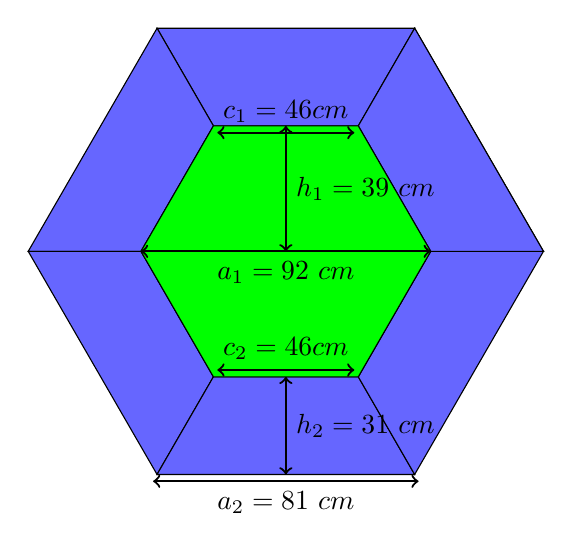
\begin{tikzpicture}
%Ich rechne mal sqrt(0.75) da hier ein gleichseitiges Dreieck vorliegt, bei dem man die Höhe berechnen muss.
%Dies geht mit dem Pythagoras, wobei der durch die Hälfte der Seite geht:
%               a²+b²=c² mit a=c/2 --> b²=c²-(c/2)²=c²-c²/4=3/4*c² --> b=c*sqrt(3/4)
%Flächenberechnung grün-blau in Python:
%R,h=50,25
%2*((2*R-R)*R*(0.75**0.5)/2)-6*((R+h*(0.75**0.5))-R)*h/2
  \pgfmathsetmacro{\hWert}{31}
  \pgfmathsetmacro{\RWert}{46}
  \pgfmathsetmacro{\dh}{\hWert/100*4}
  \pgfmathsetmacro{\R}{\RWert/100*4}
  \pgfmathsetmacro{\dR}{\dh/sqrt(0.75)}
  \pgfmathsetmacro{\hges}{(\R+\dR)*sqrt(0.75)}
  \pgfmathsetmacro{\h}{\hges-\dh}
%Schreibe ohne Komma
  \pgfmathtruncatemacro\gesamthoehe{2*(\RWert*sqrt(0.75)+\hWert)}
  \pgfmathtruncatemacro\aussenlaenge{\RWert+\hWert/sqrt(0.75)}
  \pgfmathtruncatemacro\innenlaenge{2*\RWert}
  \pgfmathtruncatemacro\innenhoehe{\RWert*sqrt(0.75)}
\foreach \rot in  {0,60,...,360}{
\draw[black,rotate=\rot,fill=blue!60] (\R,0) -- ++(\dR,0) -- ++(120:\R+\dR) -- ++(60:-\dR) -- cycle;
}
\draw[black,fill=green] (\R,0) -- ++(120:\R) -- ++(180:\R) -- ++(240:\R) -- ++(120:-\R) -- ++(0:\R) -- cycle ;
\draw[thick,<->] (-\R,0) --node[below] {$a_1=\innenlaenge~cm$} (\R,0);
\draw[thick,<->] (240:\R+\dR+0.1) --node[below] {$a_2=\aussenlaenge~cm$}  (300:\R+\dR+0.1);
\draw[thick,<->] (0,-\h) --node[right] {$h_2=\hWert~cm$} (0,-\hges);
\draw[thick,<->] (0,0) --node[right] {$h_1=\innenhoehe~cm$} (0,\h);
\draw[thick,<->] (240:\R-0.1) --node[above] {$c_2=\RWert cm$}  (300:\R-0.1);
\draw[thick,<->] (60:\R-0.1) --node[above] {$c_1=\RWert cm$}  (120:\R-0.1);
\end{tikzpicture}
$\begin{aligned}
geg.: a_1 &=92~cm& & \\
  c_1 &=46~cm& & \\
  h_1 &=140:2-31=39~cm& & \\
  a_2 &=81~cm& & \\
  c_2 &=46~cm& & \\
  h_2 &=31~cm & \\
ges.: A_{Gruen} &=?~cm^2& & \\
 A_{Blau} &=?~cm^2& & \\
& & & \\
A_{Gruen}&= 2\cdot (\frac12(a_1+c_1)\cdot h_1) & & \\
&= 2\cdot (\frac12(92+46)\cdot 39) & & \\
\makebox[0pt][l]{\uuline{\phantom{$A_{Gruen}=5.382~cm^2   \\$} } }
A_{Gruen}&=5.382~cm^2 & & \\
& & & \\
A_{blau}&= 6\cdot (\frac12(a_2+c_2)\cdot h_2) & & \\
&= 6\cdot (\frac12(81+46)\cdot 31) & & \\
\makebox[0pt][l]{\uuline{\phantom{$A_{blau}=11.885~cm^2   \\$} } }
A_{blau}&=11.885~cm^2 & & \\
\end{aligned}$
Die blaue Fläche ist größer.
}
\\\hline
b)&\pbox{7cm}{
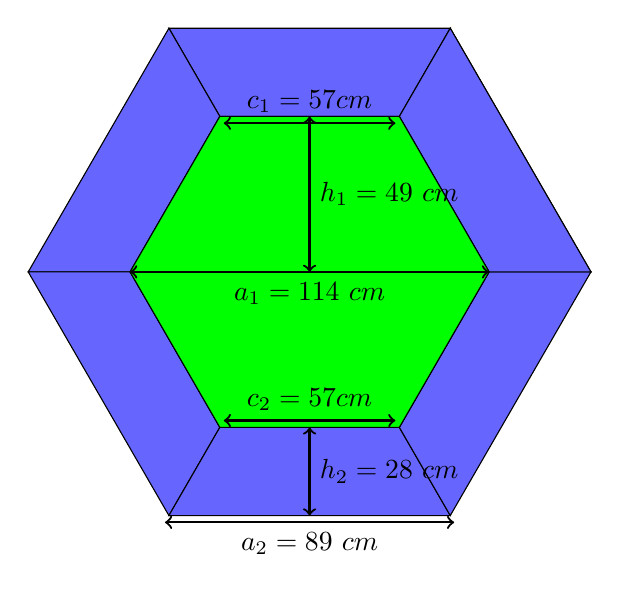
\begin{tikzpicture}
%Ich rechne mal sqrt(0.75) da hier ein gleichseitiges Dreieck vorliegt, bei dem man die Höhe berechnen muss.
%Dies geht mit dem Pythagoras, wobei der durch die Hälfte der Seite geht:
%               a²+b²=c² mit a=c/2 --> b²=c²-(c/2)²=c²-c²/4=3/4*c² --> b=c*sqrt(3/4)
%Flächenberechnung grün-blau in Python:
%R,h=50,25
%2*((2*R-R)*R*(0.75**0.5)/2)-6*((R+h*(0.75**0.5))-R)*h/2
  \pgfmathsetmacro{\hWert}{28}
  \pgfmathsetmacro{\RWert}{57}
  \pgfmathsetmacro{\dh}{\hWert/100*4}
  \pgfmathsetmacro{\R}{\RWert/100*4}
  \pgfmathsetmacro{\dR}{\dh/sqrt(0.75)}
  \pgfmathsetmacro{\hges}{(\R+\dR)*sqrt(0.75)}
  \pgfmathsetmacro{\h}{\hges-\dh}
%Schreibe ohne Komma
  \pgfmathtruncatemacro\gesamthoehe{2*(\RWert*sqrt(0.75)+\hWert)}
  \pgfmathtruncatemacro\aussenlaenge{\RWert+\hWert/sqrt(0.75)}
  \pgfmathtruncatemacro\innenlaenge{2*\RWert}
  \pgfmathtruncatemacro\innenhoehe{\RWert*sqrt(0.75)}
\foreach \rot in  {0,60,...,360}{
\draw[black,rotate=\rot,fill=blue!60] (\R,0) -- ++(\dR,0) -- ++(120:\R+\dR) -- ++(60:-\dR) -- cycle;
}
\draw[black,fill=green] (\R,0) -- ++(120:\R) -- ++(180:\R) -- ++(240:\R) -- ++(120:-\R) -- ++(0:\R) -- cycle ;
\draw[thick,<->] (-\R,0) --node[below] {$a_1=\innenlaenge~cm$} (\R,0);
\draw[thick,<->] (240:\R+\dR+0.1) --node[below] {$a_2=\aussenlaenge~cm$}  (300:\R+\dR+0.1);
\draw[thick,<->] (0,-\h) --node[right] {$h_2=\hWert~cm$} (0,-\hges);
\draw[thick,<->] (0,0) --node[right] {$h_1=\innenhoehe~cm$} (0,\h);
\draw[thick,<->] (240:\R-0.1) --node[above] {$c_2=\RWert cm$}  (300:\R-0.1);
\draw[thick,<->] (60:\R-0.1) --node[above] {$c_1=\RWert cm$}  (120:\R-0.1);
\end{tikzpicture}
$\begin{aligned}
geg.: a_1 &=114~cm& & \\
  c_1 &=57~cm& & \\
  h_1 &=154:2-28=49~cm& & \\
  a_2 &=89~cm& & \\
  c_2 &=57~cm& & \\
  h_2 &=28~cm & \\
ges.: A_{Gruen} &=?~cm^2& & \\
 A_{Blau} &=?~cm^2& & \\
& & & \\
A_{Gruen}&= 2\cdot (\frac12(a_1+c_1)\cdot h_1) & & \\
&= 2\cdot (\frac12(114+57)\cdot 49) & & \\
\makebox[0pt][l]{\uuline{\phantom{$A_{Gruen}=8.379~cm^2   \\$} } }
A_{Gruen}&=8.379~cm^2 & & \\
& & & \\
A_{blau}&= 6\cdot (\frac12(a_2+c_2)\cdot h_2) & & \\
&= 6\cdot (\frac12(89+57)\cdot 28) & & \\
\makebox[0pt][l]{\uuline{\phantom{$A_{blau}=12.291,86~cm^2   \\$} } }
A_{blau}&=12.291,86~cm^2 & & \\
\end{aligned}$
Die blaue Fläche ist größer.
}
\\\hline
c)&\pbox{7cm}{
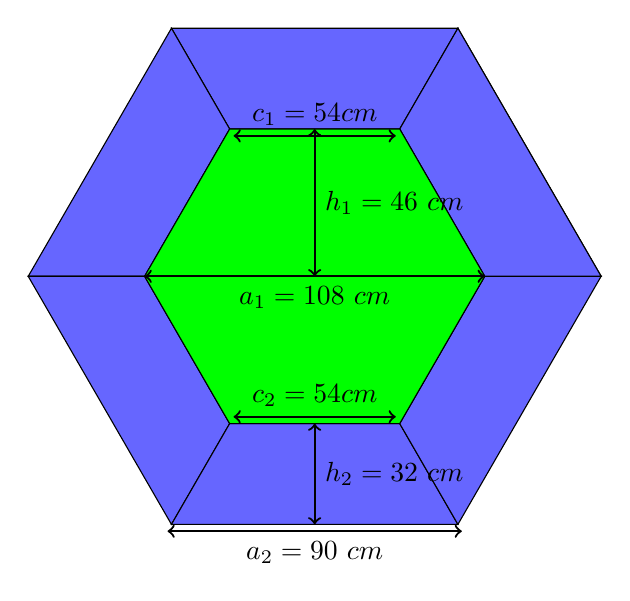
\begin{tikzpicture}
%Ich rechne mal sqrt(0.75) da hier ein gleichseitiges Dreieck vorliegt, bei dem man die Höhe berechnen muss.
%Dies geht mit dem Pythagoras, wobei der durch die Hälfte der Seite geht:
%               a²+b²=c² mit a=c/2 --> b²=c²-(c/2)²=c²-c²/4=3/4*c² --> b=c*sqrt(3/4)
%Flächenberechnung grün-blau in Python:
%R,h=50,25
%2*((2*R-R)*R*(0.75**0.5)/2)-6*((R+h*(0.75**0.5))-R)*h/2
  \pgfmathsetmacro{\hWert}{32}
  \pgfmathsetmacro{\RWert}{54}
  \pgfmathsetmacro{\dh}{\hWert/100*4}
  \pgfmathsetmacro{\R}{\RWert/100*4}
  \pgfmathsetmacro{\dR}{\dh/sqrt(0.75)}
  \pgfmathsetmacro{\hges}{(\R+\dR)*sqrt(0.75)}
  \pgfmathsetmacro{\h}{\hges-\dh}
%Schreibe ohne Komma
  \pgfmathtruncatemacro\gesamthoehe{2*(\RWert*sqrt(0.75)+\hWert)}
  \pgfmathtruncatemacro\aussenlaenge{\RWert+\hWert/sqrt(0.75)}
  \pgfmathtruncatemacro\innenlaenge{2*\RWert}
  \pgfmathtruncatemacro\innenhoehe{\RWert*sqrt(0.75)}
\foreach \rot in  {0,60,...,360}{
\draw[black,rotate=\rot,fill=blue!60] (\R,0) -- ++(\dR,0) -- ++(120:\R+\dR) -- ++(60:-\dR) -- cycle;
}
\draw[black,fill=green] (\R,0) -- ++(120:\R) -- ++(180:\R) -- ++(240:\R) -- ++(120:-\R) -- ++(0:\R) -- cycle ;
\draw[thick,<->] (-\R,0) --node[below] {$a_1=\innenlaenge~cm$} (\R,0);
\draw[thick,<->] (240:\R+\dR+0.1) --node[below] {$a_2=\aussenlaenge~cm$}  (300:\R+\dR+0.1);
\draw[thick,<->] (0,-\h) --node[right] {$h_2=\hWert~cm$} (0,-\hges);
\draw[thick,<->] (0,0) --node[right] {$h_1=\innenhoehe~cm$} (0,\h);
\draw[thick,<->] (240:\R-0.1) --node[above] {$c_2=\RWert cm$}  (300:\R-0.1);
\draw[thick,<->] (60:\R-0.1) --node[above] {$c_1=\RWert cm$}  (120:\R-0.1);
\end{tikzpicture}
$\begin{aligned}
geg.: a_1 &=108~cm& & \\
  c_1 &=54~cm& & \\
  h_1 &=156:2-32=46~cm& & \\
  a_2 &=90~cm& & \\
  c_2 &=54~cm& & \\
  h_2 &=32~cm & \\
ges.: A_{Gruen} &=?~cm^2& & \\
 A_{Blau} &=?~cm^2& & \\
& & & \\
A_{Gruen}&= 2\cdot (\frac12(a_1+c_1)\cdot h_1) & & \\
&= 2\cdot (\frac12(108+54)\cdot 46) & & \\
\makebox[0pt][l]{\uuline{\phantom{$A_{Gruen}=7.452~cm^2   \\$} } }
A_{Gruen}&=7.452~cm^2 & & \\
& & & \\
A_{blau}&= 6\cdot (\frac12(a_2+c_2)\cdot h_2) & & \\
&= 6\cdot (\frac12(90+54)\cdot 32) & & \\
\makebox[0pt][l]{\uuline{\phantom{$A_{blau}=13.915,24~cm^2   \\$} } }
A_{blau}&=13.915,24~cm^2 & & \\
\end{aligned}$
Die blaue Fläche ist größer.
}
\\\hline
d)&\pbox{7cm}{
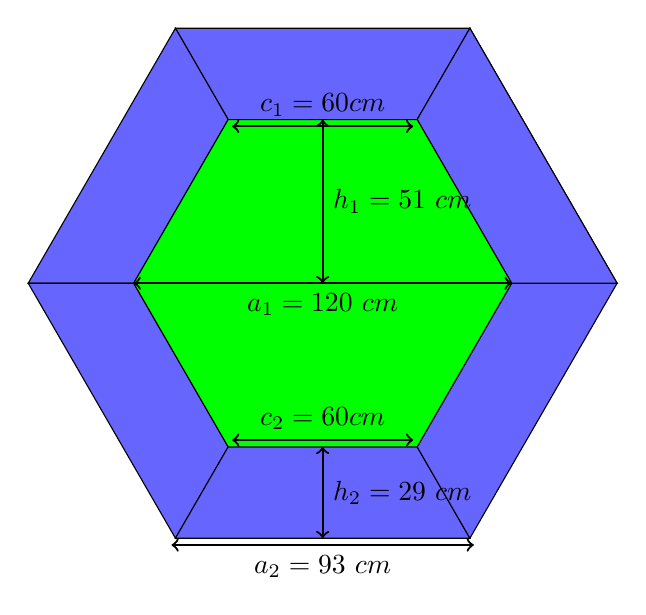
\begin{tikzpicture}
%Ich rechne mal sqrt(0.75) da hier ein gleichseitiges Dreieck vorliegt, bei dem man die Höhe berechnen muss.
%Dies geht mit dem Pythagoras, wobei der durch die Hälfte der Seite geht:
%               a²+b²=c² mit a=c/2 --> b²=c²-(c/2)²=c²-c²/4=3/4*c² --> b=c*sqrt(3/4)
%Flächenberechnung grün-blau in Python:
%R,h=50,25
%2*((2*R-R)*R*(0.75**0.5)/2)-6*((R+h*(0.75**0.5))-R)*h/2
  \pgfmathsetmacro{\hWert}{29}
  \pgfmathsetmacro{\RWert}{60}
  \pgfmathsetmacro{\dh}{\hWert/100*4}
  \pgfmathsetmacro{\R}{\RWert/100*4}
  \pgfmathsetmacro{\dR}{\dh/sqrt(0.75)}
  \pgfmathsetmacro{\hges}{(\R+\dR)*sqrt(0.75)}
  \pgfmathsetmacro{\h}{\hges-\dh}
%Schreibe ohne Komma
  \pgfmathtruncatemacro\gesamthoehe{2*(\RWert*sqrt(0.75)+\hWert)}
  \pgfmathtruncatemacro\aussenlaenge{\RWert+\hWert/sqrt(0.75)}
  \pgfmathtruncatemacro\innenlaenge{2*\RWert}
  \pgfmathtruncatemacro\innenhoehe{\RWert*sqrt(0.75)}
\foreach \rot in  {0,60,...,360}{
\draw[black,rotate=\rot,fill=blue!60] (\R,0) -- ++(\dR,0) -- ++(120:\R+\dR) -- ++(60:-\dR) -- cycle;
}
\draw[black,fill=green] (\R,0) -- ++(120:\R) -- ++(180:\R) -- ++(240:\R) -- ++(120:-\R) -- ++(0:\R) -- cycle ;
\draw[thick,<->] (-\R,0) --node[below] {$a_1=\innenlaenge~cm$} (\R,0);
\draw[thick,<->] (240:\R+\dR+0.1) --node[below] {$a_2=\aussenlaenge~cm$}  (300:\R+\dR+0.1);
\draw[thick,<->] (0,-\h) --node[right] {$h_2=\hWert~cm$} (0,-\hges);
\draw[thick,<->] (0,0) --node[right] {$h_1=\innenhoehe~cm$} (0,\h);
\draw[thick,<->] (240:\R-0.1) --node[above] {$c_2=\RWert cm$}  (300:\R-0.1);
\draw[thick,<->] (60:\R-0.1) --node[above] {$c_1=\RWert cm$}  (120:\R-0.1);
\end{tikzpicture}
$\begin{aligned}
geg.: a_1 &=120~cm& & \\
  c_1 &=60~cm& & \\
  h_1 &=160:2-29=51~cm& & \\
  a_2 &=93~cm& & \\
  c_2 &=60~cm& & \\
  h_2 &=29~cm & \\
ges.: A_{Gruen} &=?~cm^2& & \\
 A_{Blau} &=?~cm^2& & \\
& & & \\
A_{Gruen}&= 2\cdot (\frac12(a_1+c_1)\cdot h_1) & & \\
&= 2\cdot (\frac12(120+60)\cdot 51) & & \\
\makebox[0pt][l]{\uuline{\phantom{$A_{Gruen}=9.180~cm^2   \\$} } }
A_{Gruen}&=9.180~cm^2 & & \\
& & & \\
A_{blau}&= 6\cdot (\frac12(a_2+c_2)\cdot h_2) & & \\
&= 6\cdot (\frac12(93+60)\cdot 29) & & \\
\makebox[0pt][l]{\uuline{\phantom{$A_{blau}=13.353,31~cm^2   \\$} } }
A_{blau}&=13.353,31~cm^2 & & \\
\end{aligned}$
Die blaue Fläche ist größer.
}
\\\hline
e)&\pbox{7cm}{
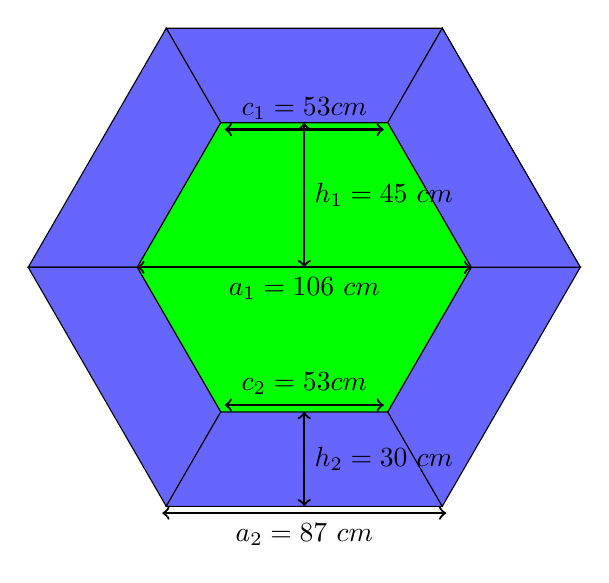
\begin{tikzpicture}
%Ich rechne mal sqrt(0.75) da hier ein gleichseitiges Dreieck vorliegt, bei dem man die Höhe berechnen muss.
%Dies geht mit dem Pythagoras, wobei der durch die Hälfte der Seite geht:
%               a²+b²=c² mit a=c/2 --> b²=c²-(c/2)²=c²-c²/4=3/4*c² --> b=c*sqrt(3/4)
%Flächenberechnung grün-blau in Python:
%R,h=50,25
%2*((2*R-R)*R*(0.75**0.5)/2)-6*((R+h*(0.75**0.5))-R)*h/2
  \pgfmathsetmacro{\hWert}{30}
  \pgfmathsetmacro{\RWert}{53}
  \pgfmathsetmacro{\dh}{\hWert/100*4}
  \pgfmathsetmacro{\R}{\RWert/100*4}
  \pgfmathsetmacro{\dR}{\dh/sqrt(0.75)}
  \pgfmathsetmacro{\hges}{(\R+\dR)*sqrt(0.75)}
  \pgfmathsetmacro{\h}{\hges-\dh}
%Schreibe ohne Komma
  \pgfmathtruncatemacro\gesamthoehe{2*(\RWert*sqrt(0.75)+\hWert)}
  \pgfmathtruncatemacro\aussenlaenge{\RWert+\hWert/sqrt(0.75)}
  \pgfmathtruncatemacro\innenlaenge{2*\RWert}
  \pgfmathtruncatemacro\innenhoehe{\RWert*sqrt(0.75)}
\foreach \rot in  {0,60,...,360}{
\draw[black,rotate=\rot,fill=blue!60] (\R,0) -- ++(\dR,0) -- ++(120:\R+\dR) -- ++(60:-\dR) -- cycle;
}
\draw[black,fill=green] (\R,0) -- ++(120:\R) -- ++(180:\R) -- ++(240:\R) -- ++(120:-\R) -- ++(0:\R) -- cycle ;
\draw[thick,<->] (-\R,0) --node[below] {$a_1=\innenlaenge~cm$} (\R,0);
\draw[thick,<->] (240:\R+\dR+0.1) --node[below] {$a_2=\aussenlaenge~cm$}  (300:\R+\dR+0.1);
\draw[thick,<->] (0,-\h) --node[right] {$h_2=\hWert~cm$} (0,-\hges);
\draw[thick,<->] (0,0) --node[right] {$h_1=\innenhoehe~cm$} (0,\h);
\draw[thick,<->] (240:\R-0.1) --node[above] {$c_2=\RWert cm$}  (300:\R-0.1);
\draw[thick,<->] (60:\R-0.1) --node[above] {$c_1=\RWert cm$}  (120:\R-0.1);
\end{tikzpicture}
$\begin{aligned}
geg.: a_1 &=106~cm& & \\
  c_1 &=53~cm& & \\
  h_1 &=150:2-30=45~cm& & \\
  a_2 &=87~cm& & \\
  c_2 &=53~cm& & \\
  h_2 &=30~cm & \\
ges.: A_{Gruen} &=?~cm^2& & \\
 A_{Blau} &=?~cm^2& & \\
& & & \\
A_{Gruen}&= 2\cdot (\frac12(a_1+c_1)\cdot h_1) & & \\
&= 2\cdot (\frac12(106+53)\cdot 45) & & \\
\makebox[0pt][l]{\uuline{\phantom{$A_{Gruen}=7.155~cm^2   \\$} } }
A_{Gruen}&=7.155~cm^2 & & \\
& & & \\
A_{blau}&= 6\cdot (\frac12(a_2+c_2)\cdot h_2) & & \\
&= 6\cdot (\frac12(87+53)\cdot 30) & & \\
\makebox[0pt][l]{\uuline{\phantom{$A_{blau}=12.657,69~cm^2   \\$} } }
A_{blau}&=12.657,69~cm^2 & & \\
\end{aligned}$
Die blaue Fläche ist größer.
}
\\\hline
f)&\pbox{7cm}{
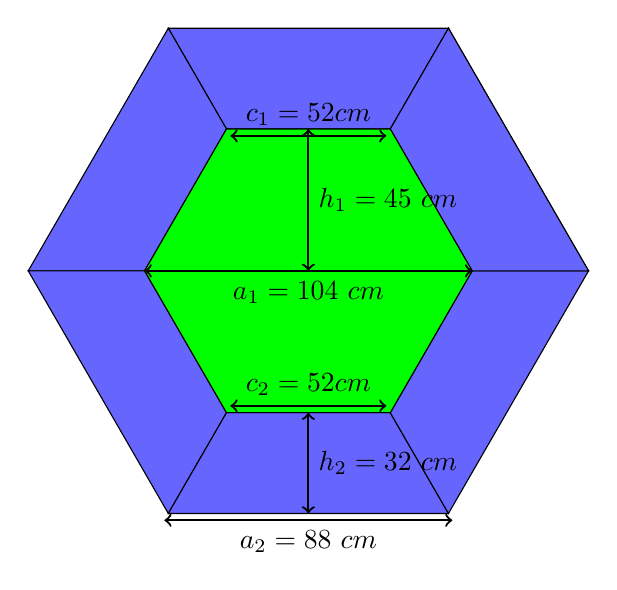
\begin{tikzpicture}
%Ich rechne mal sqrt(0.75) da hier ein gleichseitiges Dreieck vorliegt, bei dem man die Höhe berechnen muss.
%Dies geht mit dem Pythagoras, wobei der durch die Hälfte der Seite geht:
%               a²+b²=c² mit a=c/2 --> b²=c²-(c/2)²=c²-c²/4=3/4*c² --> b=c*sqrt(3/4)
%Flächenberechnung grün-blau in Python:
%R,h=50,25
%2*((2*R-R)*R*(0.75**0.5)/2)-6*((R+h*(0.75**0.5))-R)*h/2
  \pgfmathsetmacro{\hWert}{32}
  \pgfmathsetmacro{\RWert}{52}
  \pgfmathsetmacro{\dh}{\hWert/100*4}
  \pgfmathsetmacro{\R}{\RWert/100*4}
  \pgfmathsetmacro{\dR}{\dh/sqrt(0.75)}
  \pgfmathsetmacro{\hges}{(\R+\dR)*sqrt(0.75)}
  \pgfmathsetmacro{\h}{\hges-\dh}
%Schreibe ohne Komma
  \pgfmathtruncatemacro\gesamthoehe{2*(\RWert*sqrt(0.75)+\hWert)}
  \pgfmathtruncatemacro\aussenlaenge{\RWert+\hWert/sqrt(0.75)}
  \pgfmathtruncatemacro\innenlaenge{2*\RWert}
  \pgfmathtruncatemacro\innenhoehe{\RWert*sqrt(0.75)}
\foreach \rot in  {0,60,...,360}{
\draw[black,rotate=\rot,fill=blue!60] (\R,0) -- ++(\dR,0) -- ++(120:\R+\dR) -- ++(60:-\dR) -- cycle;
}
\draw[black,fill=green] (\R,0) -- ++(120:\R) -- ++(180:\R) -- ++(240:\R) -- ++(120:-\R) -- ++(0:\R) -- cycle ;
\draw[thick,<->] (-\R,0) --node[below] {$a_1=\innenlaenge~cm$} (\R,0);
\draw[thick,<->] (240:\R+\dR+0.1) --node[below] {$a_2=\aussenlaenge~cm$}  (300:\R+\dR+0.1);
\draw[thick,<->] (0,-\h) --node[right] {$h_2=\hWert~cm$} (0,-\hges);
\draw[thick,<->] (0,0) --node[right] {$h_1=\innenhoehe~cm$} (0,\h);
\draw[thick,<->] (240:\R-0.1) --node[above] {$c_2=\RWert cm$}  (300:\R-0.1);
\draw[thick,<->] (60:\R-0.1) --node[above] {$c_1=\RWert cm$}  (120:\R-0.1);
\end{tikzpicture}
$\begin{aligned}
geg.: a_1 &=104~cm& & \\
  c_1 &=52~cm& & \\
  h_1 &=154:2-32=45~cm& & \\
  a_2 &=88~cm& & \\
  c_2 &=52~cm& & \\
  h_2 &=32~cm & \\
ges.: A_{Gruen} &=?~cm^2& & \\
 A_{Blau} &=?~cm^2& & \\
& & & \\
A_{Gruen}&= 2\cdot (\frac12(a_1+c_1)\cdot h_1) & & \\
&= 2\cdot (\frac12(104+52)\cdot 45) & & \\
\makebox[0pt][l]{\uuline{\phantom{$A_{Gruen}=7.020~cm^2   \\$} } }
A_{Gruen}&=7.020~cm^2 & & \\
& & & \\
A_{blau}&= 6\cdot (\frac12(a_2+c_2)\cdot h_2) & & \\
&= 6\cdot (\frac12(88+52)\cdot 32) & & \\
\makebox[0pt][l]{\uuline{\phantom{$A_{blau}=13.531,24~cm^2   \\$} } }
A_{blau}&=13.531,24~cm^2 & & \\
\end{aligned}$
Die blaue Fläche ist größer.
}
\\\hline
g)&\pbox{7cm}{
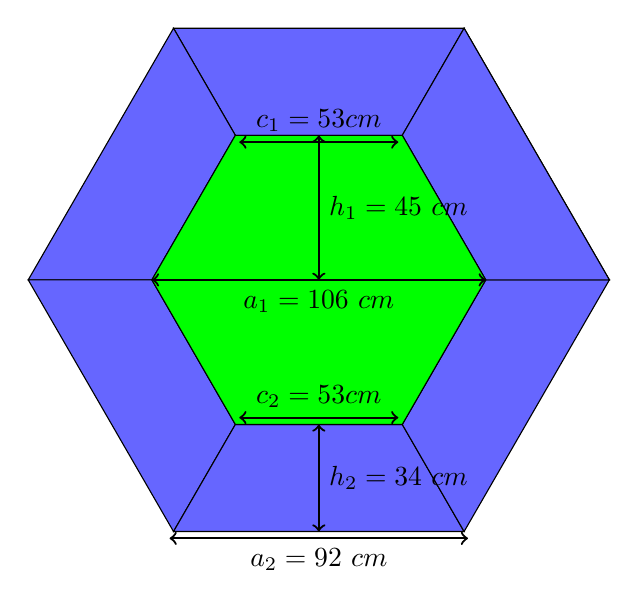
\begin{tikzpicture}
%Ich rechne mal sqrt(0.75) da hier ein gleichseitiges Dreieck vorliegt, bei dem man die Höhe berechnen muss.
%Dies geht mit dem Pythagoras, wobei der durch die Hälfte der Seite geht:
%               a²+b²=c² mit a=c/2 --> b²=c²-(c/2)²=c²-c²/4=3/4*c² --> b=c*sqrt(3/4)
%Flächenberechnung grün-blau in Python:
%R,h=50,25
%2*((2*R-R)*R*(0.75**0.5)/2)-6*((R+h*(0.75**0.5))-R)*h/2
  \pgfmathsetmacro{\hWert}{34}
  \pgfmathsetmacro{\RWert}{53}
  \pgfmathsetmacro{\dh}{\hWert/100*4}
  \pgfmathsetmacro{\R}{\RWert/100*4}
  \pgfmathsetmacro{\dR}{\dh/sqrt(0.75)}
  \pgfmathsetmacro{\hges}{(\R+\dR)*sqrt(0.75)}
  \pgfmathsetmacro{\h}{\hges-\dh}
%Schreibe ohne Komma
  \pgfmathtruncatemacro\gesamthoehe{2*(\RWert*sqrt(0.75)+\hWert)}
  \pgfmathtruncatemacro\aussenlaenge{\RWert+\hWert/sqrt(0.75)}
  \pgfmathtruncatemacro\innenlaenge{2*\RWert}
  \pgfmathtruncatemacro\innenhoehe{\RWert*sqrt(0.75)}
\foreach \rot in  {0,60,...,360}{
\draw[black,rotate=\rot,fill=blue!60] (\R,0) -- ++(\dR,0) -- ++(120:\R+\dR) -- ++(60:-\dR) -- cycle;
}
\draw[black,fill=green] (\R,0) -- ++(120:\R) -- ++(180:\R) -- ++(240:\R) -- ++(120:-\R) -- ++(0:\R) -- cycle ;
\draw[thick,<->] (-\R,0) --node[below] {$a_1=\innenlaenge~cm$} (\R,0);
\draw[thick,<->] (240:\R+\dR+0.1) --node[below] {$a_2=\aussenlaenge~cm$}  (300:\R+\dR+0.1);
\draw[thick,<->] (0,-\h) --node[right] {$h_2=\hWert~cm$} (0,-\hges);
\draw[thick,<->] (0,0) --node[right] {$h_1=\innenhoehe~cm$} (0,\h);
\draw[thick,<->] (240:\R-0.1) --node[above] {$c_2=\RWert cm$}  (300:\R-0.1);
\draw[thick,<->] (60:\R-0.1) --node[above] {$c_1=\RWert cm$}  (120:\R-0.1);
\end{tikzpicture}
$\begin{aligned}
geg.: a_1 &=106~cm& & \\
  c_1 &=53~cm& & \\
  h_1 &=158:2-34=45~cm& & \\
  a_2 &=92~cm& & \\
  c_2 &=53~cm& & \\
  h_2 &=34~cm & \\
ges.: A_{Gruen} &=?~cm^2& & \\
 A_{Blau} &=?~cm^2& & \\
& & & \\
A_{Gruen}&= 2\cdot (\frac12(a_1+c_1)\cdot h_1) & & \\
&= 2\cdot (\frac12(106+53)\cdot 45) & & \\
\makebox[0pt][l]{\uuline{\phantom{$A_{Gruen}=7.155~cm^2   \\$} } }
A_{Gruen}&=7.155~cm^2 & & \\
& & & \\
A_{blau}&= 6\cdot (\frac12(a_2+c_2)\cdot h_2) & & \\
&= 6\cdot (\frac12(92+53)\cdot 34) & & \\
\makebox[0pt][l]{\uuline{\phantom{$A_{blau}=14.816,5~cm^2   \\$} } }
A_{blau}&=14.816,5~cm^2 & & \\
\end{aligned}$
Die blaue Fläche ist größer.
}
\\\hline
h)&\pbox{7cm}{
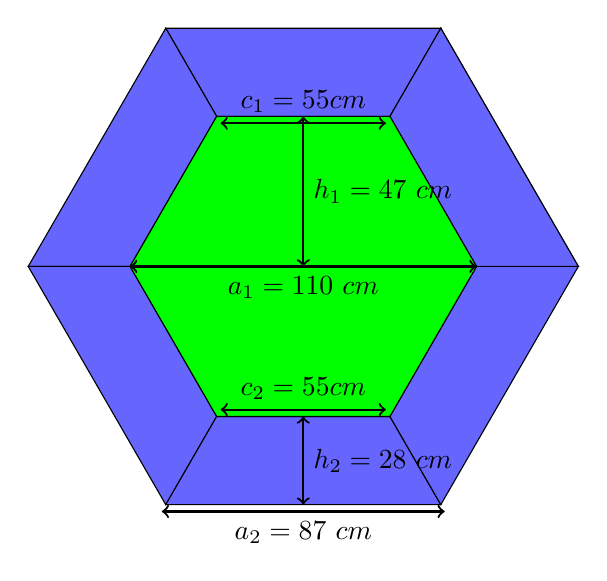
\begin{tikzpicture}
%Ich rechne mal sqrt(0.75) da hier ein gleichseitiges Dreieck vorliegt, bei dem man die Höhe berechnen muss.
%Dies geht mit dem Pythagoras, wobei der durch die Hälfte der Seite geht:
%               a²+b²=c² mit a=c/2 --> b²=c²-(c/2)²=c²-c²/4=3/4*c² --> b=c*sqrt(3/4)
%Flächenberechnung grün-blau in Python:
%R,h=50,25
%2*((2*R-R)*R*(0.75**0.5)/2)-6*((R+h*(0.75**0.5))-R)*h/2
  \pgfmathsetmacro{\hWert}{28}
  \pgfmathsetmacro{\RWert}{55}
  \pgfmathsetmacro{\dh}{\hWert/100*4}
  \pgfmathsetmacro{\R}{\RWert/100*4}
  \pgfmathsetmacro{\dR}{\dh/sqrt(0.75)}
  \pgfmathsetmacro{\hges}{(\R+\dR)*sqrt(0.75)}
  \pgfmathsetmacro{\h}{\hges-\dh}
%Schreibe ohne Komma
  \pgfmathtruncatemacro\gesamthoehe{2*(\RWert*sqrt(0.75)+\hWert)}
  \pgfmathtruncatemacro\aussenlaenge{\RWert+\hWert/sqrt(0.75)}
  \pgfmathtruncatemacro\innenlaenge{2*\RWert}
  \pgfmathtruncatemacro\innenhoehe{\RWert*sqrt(0.75)}
\foreach \rot in  {0,60,...,360}{
\draw[black,rotate=\rot,fill=blue!60] (\R,0) -- ++(\dR,0) -- ++(120:\R+\dR) -- ++(60:-\dR) -- cycle;
}
\draw[black,fill=green] (\R,0) -- ++(120:\R) -- ++(180:\R) -- ++(240:\R) -- ++(120:-\R) -- ++(0:\R) -- cycle ;
\draw[thick,<->] (-\R,0) --node[below] {$a_1=\innenlaenge~cm$} (\R,0);
\draw[thick,<->] (240:\R+\dR+0.1) --node[below] {$a_2=\aussenlaenge~cm$}  (300:\R+\dR+0.1);
\draw[thick,<->] (0,-\h) --node[right] {$h_2=\hWert~cm$} (0,-\hges);
\draw[thick,<->] (0,0) --node[right] {$h_1=\innenhoehe~cm$} (0,\h);
\draw[thick,<->] (240:\R-0.1) --node[above] {$c_2=\RWert cm$}  (300:\R-0.1);
\draw[thick,<->] (60:\R-0.1) --node[above] {$c_1=\RWert cm$}  (120:\R-0.1);
\end{tikzpicture}
$\begin{aligned}
geg.: a_1 &=110~cm& & \\
  c_1 &=55~cm& & \\
  h_1 &=150:2-28=47~cm& & \\
  a_2 &=87~cm& & \\
  c_2 &=55~cm& & \\
  h_2 &=28~cm & \\
ges.: A_{Gruen} &=?~cm^2& & \\
 A_{Blau} &=?~cm^2& & \\
& & & \\
A_{Gruen}&= 2\cdot (\frac12(a_1+c_1)\cdot h_1) & & \\
&= 2\cdot (\frac12(110+55)\cdot 47) & & \\
\makebox[0pt][l]{\uuline{\phantom{$A_{Gruen}=7.755~cm^2   \\$} } }
A_{Gruen}&=7.755~cm^2 & & \\
& & & \\
A_{blau}&= 6\cdot (\frac12(a_2+c_2)\cdot h_2) & & \\
&= 6\cdot (\frac12(87+55)\cdot 28) & & \\
\makebox[0pt][l]{\uuline{\phantom{$A_{blau}=11.955,86~cm^2   \\$} } }
A_{blau}&=11.955,86~cm^2 & & \\
\end{aligned}$
Die blaue Fläche ist größer.
}
\\\hline
\end{xltabular}
\vspace{0.5cm}
\end{document}